%% Basierend auf einer TeXnicCenter-Vorlage von Mark M�ller
%%%%%%%%%%%%%%%%%%%%%%%%%%%%%%%%%%%%%%%%%%%%%%%%%%%%%%%%%%%%%%%%%%%%%%%

% W�hlen Sie die Optionen aus, indem Sie % vor der Option entfernen  
% Dokumentation des KOMA-Script-Packets: scrguide

%%%%%%%%%%%%%%%%%%%%%%%%%%%%%%%%%%%%%%%%%%%%%%%%%%%%%%%%%%%%%%%%%%%%%%%
%% Optionen zum Layout des Artikels                                  %%
%%%%%%%%%%%%%%%%%%%%%%%%%%%%%%%%%%%%%%%%%%%%%%%%%%%%%%%%%%%%%%%%%%%%%%%
\documentclass[%
%a5paper,							% alle weiteren Papierformat einstellbar
%landscape,						% Querformat
%10pt,								% Schriftgr��e (12pt, 11pt (Standard))
%BCOR1cm,							% Bindekorrektur, bspw. 1 cm
%DIVcalc,							% f�hrt die Satzspiegelberechnung neu aus
%											  s. scrguide 2.4
%twoside,							% Doppelseiten
%twocolumn,						% zweispaltiger Satz
%halfparskip*,				% Absatzformatierung s. scrguide 3.1
%headsepline,					% Trennline zum Seitenkopf	
%footsepline,					% Trennline zum Seitenfu�
titlepage,						% Titelei auf eigener Seite
%normalheadings,			% �berschriften etwas kleiner (smallheadings)
%idxtotoc,						% Index im Inhaltsverzeichnis
%liststotoc,					% Abb.- und Tab.verzeichnis im Inhalt
%bibtotoc,						% Literaturverzeichnis im Inhalt
%abstracton,					% �berschrift �ber der Zusammenfassung an	
%leqno,   						% Nummerierung von Gleichungen links
%fleqn,								% Ausgabe von Gleichungen linksb�ndig
%draft								% �berlangen Zeilen in Ausgabe gekennzeichnet
]
{scrartcl} 

%\pagestyle{empty}		% keine Kopf und Fu�zeile (k. Seitenzahl)
\pagestyle{headings}	% lebender Kolumnentitel  


%% Deutsche Anpassungen %%%%%%%%%%%%%%%%%%%%%%%%%%%%%%%%%%%%%
\usepackage[ngerman]{babel}
\usepackage[T1]{fontenc}
\usepackage[ansinew]{inputenc}
\usepackage{amsmath}
\usepackage{lmodern} %Type1-Schriftart f�r nicht-englische Texte
\usepackage{siunitx}
%\usepackage{}

%% Packages f�r Grafiken & Abbildungen %%%%%%%%%%%%%%%%%%%%%%
\usepackage{graphicx} %%Zum Laden von Grafiken
\usepackage{subfig} %%Teilabbildungen in einer Abbildung
%\usepackage{pst-all} %%PSTricks - nicht verwendbar mit pdfLaTeX

%% Beachten Sie:
%% 
%% Im Modus "LaTeX => PDF" k�nnen Sie u.a. folgende Grafikformate verwenden:
%%   .jpg  .png  .pdf  .mps
%% 
%% In den Modi "LaTeX => DVI", "LaTeX => PS" und "LaTeX => PS => PDF"
%% k�nnen Sie u.a. folgende Grafikformate verwenden:
%%   .eps  .ps  .bmp  .pict  .pntg



\begin{document}

%\pagestyle{empty} %%Keine Kopf-/Fusszeilen auf den ersten Seiten.


%% Angaben zur Standardformatierung des Titels %%%%%%%%%%%%%%%%%%%%%%%%
%\titlehead{Titelkopf }
\subject{Einf�hrung in die Medizinische Physik}
\title{Praktikumsprotokoll: Audiometrie}
\author{Sarah Schmetkamp (xxxxxxx)\\Jan Lietz (xxxxxxx) \\Lukas K�pper(2444460)}

\date{05.01.2016}				
\maketitle 						% Titelei wird erzeugt

 \section{Aufbau und Funktion des Ohrs}
Das menschliche Geh�r kann T�ne nur innerhalb eines bestimmten Frequenz- und Schalldruckpegelbereichs wahrnehmen. Die H�rschwelle liegt bei einer Frequenz von $\SI{1.000}{Hz}$ etwa bei $\SI{0}{dB-SPL}$. Die Schmerzgrenze liegt bei etwa $\SI{120}{dB-SPL}$. Der Freuenzbereich erstreckt sich von ca. $\SI{20}{Hz}$ bis ca. $\SI{20000}{Hz}$.

\begin{figure}[h]
 \centering
  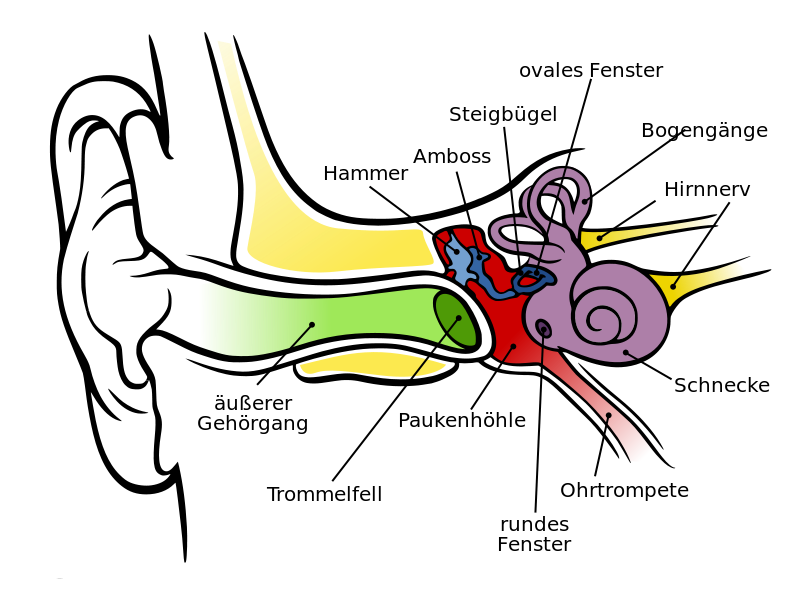
\includegraphics[width=\textwidth]{../Bilder/Ohr.png}
 \caption{Aufbau des Ohrs. Chittka L, Brockmann}
 \label{fig:lineareAnpassung} 
\end{figure} 




Das Ohr l�sst sich in die drei Bereiche Au�enohr, Mittelohr und Innenohr gliedern.

Das Au�enohr besteht aus Ohrmuschel und dem �u�eren Geh�rgang. Seine Hauptaufgabe ist das Auffangen und Weiterleiten des Schalls zum Trommelfell. Durch die unsymmetrische Form der Ohrmuschel, ist eine Richtungsbestimmung des Schalls m�glich. Die Richtungsaufl�sung geschieht jedoch haupts�chlich �ber Laufzeit- und Lautst�rkeunterschiede zwischen beiden Ohren. Au�erdem dient das Au�enohr dem Schutz der empfindlichen Bestandteile im Mittel- und Innenohr.

Das Mittelohr wird nach au�en vom Trommelfell und nach innen vom ovalen und runden Fenster begrenzt. Die Funktion des Mittelohres besteht in der Impedanzanpassung zwischen dem Schall in Luft (Au�enohr) und dem Schall in der Perilymphe (Innenohr). Die Geh�rkn�chelchen Hammer, Amboss und Steigb�gel bilden ein Hebelsystem, dass die Auslenkung vom Trommelfell zum ovalen Fenster �bertr�gt und dabei verst�rkt. Durch die unterschiedliche Fl�che von Trommelfell und ovalem Fenster und die Hebelwirkung der Geh�rkn�chelchen ergibt sich eine Druckverst�rkung von etwa $26$. Die Eustachische R�hre verbindet Mittelohr und Nasenrachenraum. Sie erm�glicht einen Druckausgleich, der durch wechselnden Au�endruck n�tig wird.

Das Innenohr ist in ein Hohlraumsystem innerhalb des Schl�fenbeins eingebettet. Den oberen Teil des Innenohr bildet das Gleichgewichtsorgan (Labyrinth). Es besteht aus drei zueinander senkrecht stehenden Schleifen und dient dem Erkennen von Bewegungs�nderungen und der Richtung der Erdanziehungskraft. Der untere Teil beinhaltet die Cochlea. Ihre Aufgaben bestehen in der Umwandlung des Drucksignals in elektrische Signale und der Weiterleitung an die Nervenbahnen. Die Cochlea ist durch die Basilarmembran l�ngs in zwei Bereiche geteilt. Haarzellen auf der Basilarmembran werden durch die Bewegung der Lymphe gebogen und l�sen dabei Nervenimpulse aus. Durch eine Orstkodierung kann dabei die Frequenz des einlaufenden Schalls ermittelt werden.


Die Techniken zur Untersuchung der H�rf�higkeit werden unter dem Begriff Audiometrie zusammengefasst. Das Ergebnis eines H�rtests, der das H�rverm�gen bei verschiedenen Frequenzen untersucht, nennt sich Audiogramm.

\section{Durchf�hrung}
\subsection{Analoges Audiogramm}
Im ersten Versuchsteil wird mit einem analogen Audiometer von Oscilla ein Audiogramm erstellt. Der Proband sitzt mit dem R�cken zum Ger�t, um m�glichst wenig beeinflusst zu werden. Nun werden zun�chst f�r das rechte Ohr und anschlie�end f�r das linke Ohr nacheinander $11$ voreingestellt Frequenzen zwischen $\SI{125}{Hz}$ und $\SI{8}{kHz}$ durch den Kopfh�rer wiedergegeben. Sobald der Proband einen Ton h�rt, signalisiert er dies �ber einen Dr�cker. Der Versuchsleiter notiert daraufhin den jeweiligen Wert.

Diese Messung wird f�r drei Probanden durchgef�hrt.


\subsection{Digitales Audiogramm}
Im zweiten Versuchsteil wird das digitale Audiometer Oscilla USB-350B verwendet, um ein Audiogramm zu erstellen. Die Messung erfolgt parallel zum ersten Versuchsteil. Der Computer ermittelt hierbei jedoch die H�rschwelle f�r die $11$ Frequenzen selbstst�ndig nach dem Hughson-Westlake-Test.

\subsection{Digitales Audiogramm der Knochenleitung}
In diesem Versuchsteil soll die H�rschwelle f�r Knochenschall bestimmt werden. Der Tongeber wird auf das Schl�fenbein am rechten bzw. linken Ohr gesetzt. Zus�tzlich tr�gt der Proband Kopfh�rer, die das Ohr abschirmen, den Tongeber jedoch nicht einschlie�en. Wieder erfolgt die Bestimmung der H�rschwelle manuell f�r $?$ verschiedene Frequenzen.

Die beiden Digitalen Audiogramme werden f�r den selben Probanden erstellt.

\subsection{Ausf�hrliches Audiogramm}
Mithilfe eines Funktionsgenerators wird die H�rschwelle f�r $54$ Frequenzen zwischen $\SI{80}{Hz}$ und $\SI{18}{kHz}$ zun�chst f�r das rechte und anschlie�end f�r das linke Ohr ermittelt.

\subsection{Ausf�hrliches Audiogramm mit St�rquelle}
Es erfolgt eine Messung der H�rschwelle f�r $?$ Frequenzen zwischen $\SI{80}{Hz}$ und $\SI{18}{kHz}$. Hierbei wird jedoch ein Rauschen als St�rsignal mit einem zweiten Funktionsgenerator erzeugt und ebenfalls in den Kopfh�rer gespielt. Die ERstellung des Audiogramms erfolgt zun�chst mit einem Str�rrauschen von $\SI{}{dB}$ und dann mit $\SI{}{dB}$.

\section{Auswertung der Audiogramme}

Die Auswertung und die Darstellung der durchgef�hrten Audiogramme erfolgt mit \texttt{Python} und den Paketen \texttt{Numpy, Scipy} und \texttt{Matplotlib}.

\subsection{Analoges Audiogramm}

\begin{figure}[h]
	\centering
		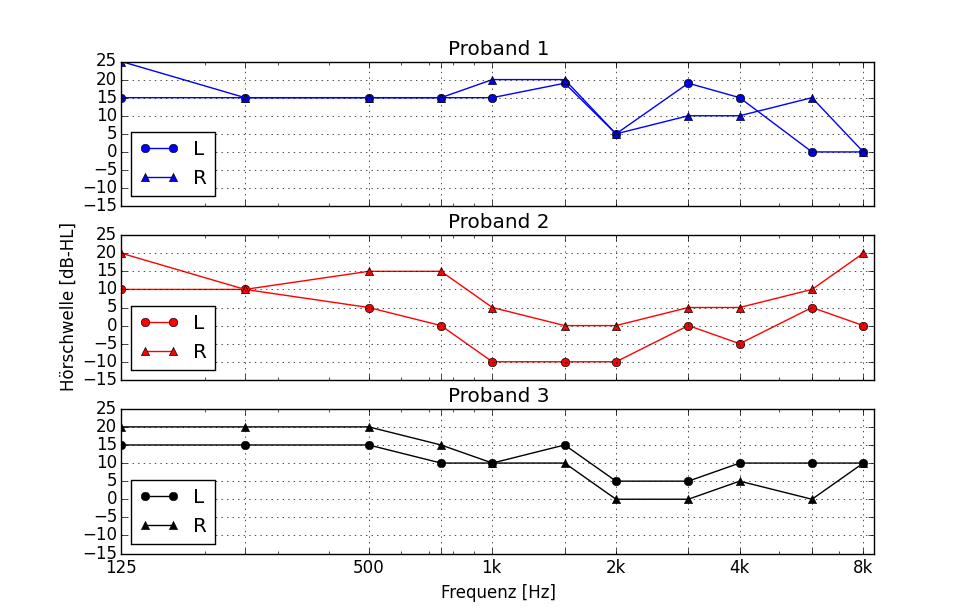
\includegraphics[width=0.85\textwidth]{../Bilder/man_audio1.png}
	\caption{Analoge Audiogramme der drei Probanden. }
	\label{fig:man_audio1}
\end{figure}

In Abb. \ref{fig:man_audio1} sind die aufgenommenen Audiogramme der drei Probanden dargestellt. Die Genauigkeit der Werte l�sst sich hierbei auf $\pm \SI{2,5}{dB-HL}$ absch�tzen, da das Ger�t nur eine Lautst�rke-Variation in $\SI{5}{dB-HL}$-Schritten zul�sst. Man kann erkennen, dass alle drei Probanden �ber den gesamten Frequenzbereich im normalen Bereich liegen. Proband 1 zeigt �ber den gesamten getesteten Frequenzbereich relativ konstant im Bereich um $\SI{10}{dB-HL}$ und damit etwas unter dem Durchschnitt. Proband 2 hingegen liegt beim linken Ohr auf einem gro�en Frequenzbereich unter $\SI{0}{dB-HL}$ und damit besser als der Durchschnitt. Auf dem rechten Ohr ist die Tonwahrnehmung �ber fast den gesamten Frequenzbereich schlechter. Dies k�nnte dadurch zu Stande gekommen sein, dass die verwendeten Kopfh�rer scheinbar einen Defekt am rechten H�rer haben, wie sich im dritten Versuchsteil herausgestellt hat. Dagegen spricht allerdings, dass sich diese Systematik nicht so stark bei den anderen beiden Probanden feststellen l�sst. Zusammenfassend l�sst sich sagen, dass Proband 2 das beste Geh�r hat und alle Probanden eine gesunde Tonwahrnehmung im getesteten Frequenzbereich haben.

\subsection{Digitales Audiogramm}

\begin{figure}[h]
	\centering
		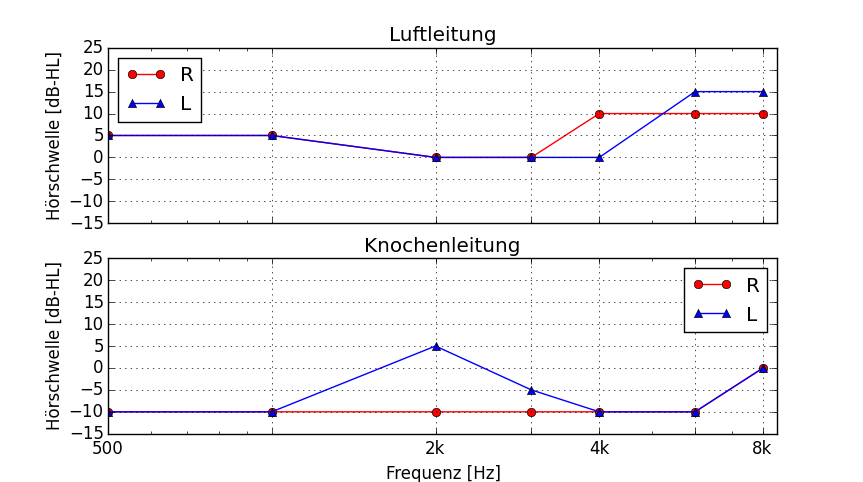
\includegraphics[width=0.85\textwidth]{../Bilder/man_audio_knochen.png}
	\caption{Digital aufgezeichnete Audiogramme f�r Luftleitung und Knochenleitung}
	\label{fig:man_audio_knochen}
\end{figure}

In Abb. \ref{fig:man_audio_knochen} sind die automatisch aufgenommenen Audiogramme f�r das rechte und linke Ohr und die manuell aufgenommenen Audiogramme der Knochenleitung von Proband 3 dargsetellt. Die automatische Aufnahme der Audiogramme der Luftleitung erfolgt nach dem Hughson-Westlake Test. Hierbei wird die Lautst�rke der Testt�ne mehrmals bei einer fixen Frequenz variiert, um eine h�here Sicherheit bei der Bestimmung der H�rschwelle des Probanden zu erreichen. Obwohl auch dieses Ger�t nur eine Lautst�rke-Variation von $\SI{5}{dB-HL}$ erm�glicht, l�sst sich eine Diskrepanz zwischen dem im ersten Versuchsteil aufgenommenen Audiogramm und dem digital aufgenommenen Audiogramm erkennen. Proband 3 zeigt in dem getesteten Frequenzbereich keinen signifikanten Unterschied zwischen linkem und rechtem Ohr und die Werte f�r die H�rschwelle liegen n�her an der Normschwelle von $\SI{0}{dB-HL}$. Nur im hochfrequenten Bereich gibt es eine leichte Abweichung nach oben. \\

\subsubsection{Knochenleitung}

Bei der Bestimmung der Knochenleitung ist anzumerken, dass das Ger�t eine minimale Lautst�rke-Einstellung von $\SI{-10}{dB-HL}$ erm�glicht. Dementsprechend kann f�r das rechte Ohr auf dem gesamten Frequenzbereich nur eine obere Grenze der H�rschwelle angegeben werden. Lediglich bei $\SI{2}{kHz}$ und $\SI{3}{kHz}$ beim Audiogramm des linken Ohres musste die Lautst�rke erh�ht werden, damit der Proband den Ton wahrnehmen konnte. Ebenfalls ist anzumerken, dass die maximal einzustellende Tonfrequenz beim Knochenleitungsaudiogramm $\SI{6}{kHz}$ ist. 


\subsection{Ausf�hrliches Audiogramm}

Zur Aufnahme des detaillierten Audiogramms von Proband 2 wird ein Frequenzgenerator benutzt, der ein Sinus-Signal mit variabler Spannungsamplitude ausgibt. Dieser Generator wird �ber ein Mischpult an die im ersten Versuchsteil verwendeten Kopfh�rer angeschlossen. Um ein aussagekr�ftiges Audiogramm aufzunehmen, muss zun�chst das vom Frequenzgenerator ausgegebene Signal in ein auf die Schallintensit�t bezogenes Signal umgerechnet werden. Der Frequenzgenerator gibt die Signalintensit�t in der Einheit $\mbox{dB V}$ aus. Es ist anzumerken, dass im Gegensatz zur Konvention, $\SI{20}{dB-V}$ einer Verdopplung der Signalintensit�t am Frequenzgenerator entspricht. Dementsprechend muss zun�chst, um die �bliche Skalierung der Schallintensit�t zu erreichen, der Signalwert halbiert werden. 
Es wird davon ausgegangen, dass das Headset eine lineare �bersetzung von eingehendem Spannungssignal in ausgehendes Schallsignal unabh�ngig von der anregenden Frequenz vollbringt. F�r diesen Fall erfolgt die Umrechnung durch einen konstanten Offset. Diesen Offset erh�lt man durch den Vergleich des detaillierten Audiogramms mit dem im ersten Versuchsteil aufgenommenen Audiogramms. Zur Ermittlung des Offsets wird der Referenzwert bei $\SI{1}{kHz}$ verwendet, da f�r diese Frequenz ebenfalls der Wert in $\mbox{dB-SPL}$ dem Wert in $\mbox{dB-HL}$ entspricht. Es wird der Wert des linken Ohres von Proband 2 im ersten Versuch als Offset $c_{Off}$ zwischen $\mbox{dB-SPL}$ und $\mbox{dB-V}$ angenommen. 
%
\begin{equation}
		I[\mbox{dB-SPL}] = I[\mbox{dB-V}] +c_{off}  \quad \mbox{ mit } c_{off} = \SI{34}{dB}
		\label{eq:SPL_offset}
\end{equation}

Dieser Offset wird auf die $\mbox{dB-V}$ Kurve addiert, um die $\mbox{dB-SPL}$ Kurve zu erhalten. \\


\begin{figure}[htbp]
	\centering
		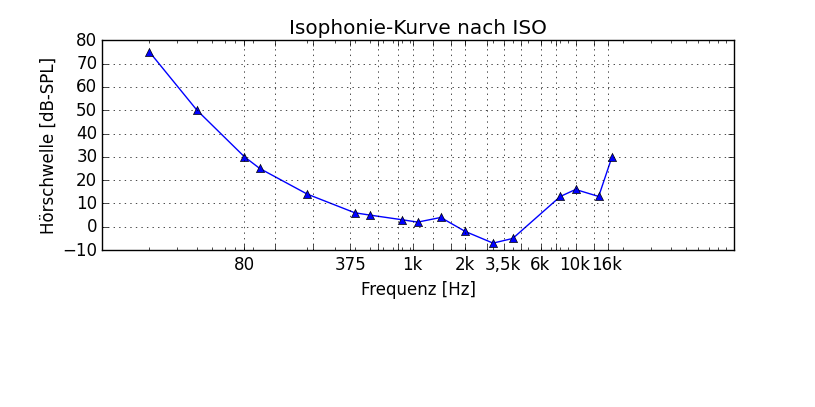
\includegraphics[width=1.00\textwidth]{../Bilder/isophonie_kurve.png}
	\caption{Isophonie Kurve f�r die H�rschwelle. Daten entnommen aus ISO 226:2003}
	\label{fig:isophonie_kurve}
\end{figure}



Um aus dieser Kurve das Audiogramm in der Einheit $\mbox{dB-HL}$ zu erhalten muss die Kurve noch auf die Empfindlichkeit des menschlichen Geh�rs normiert werden. F�r diese Normierung wird die Isophonie-Kurve der H�rschwelle aus der ISO-Norm ISO 226:2003(Abb. \ref{fig:isophonie_kurve}) verwendet. 
Die Punktdichte dieser Kurve ist zu niedrig, um f�r alle im Audiogramm getesteten Frequenzen einen eigenen Anpassungswert zu liefern. Um dennoch eine Umrechnung zwischen $\mbox{dB-SPL}$ in $\mbox{dB-HL}$ zu erm�glichen, wird zwischen den Werten der Isophonie-Kurve interpoliert. Es wird eine im Logarithmus der Frequenz lineare Interpolation verwendet, sodass sich f�r eine Frequenz $f_x$, die sich zwischen zwei Frequenzpunkten $f_i$ und $f_{i+1}$ befindet, eine Korrektur $\Delta I_{HL}(f_x)$ ergibt:

\begin{align*}
	\Delta I_{HL}(f_x) &= m \cdot \ln{f_x} + n \\
	\mbox{mit}\quad m &= \frac{\Delta I_{HL}(f_{i+1})-\Delta I_{HL}(f_{i})}{\ln{f_{i+1}} - \ln{f_{i}}} \\
	\mbox{und}\quad n &= \Delta I_{HL}(f_{i}) - m\cdot \ln{f_i}
\end{align*}

Es ergibt sich also insgesamt f�r das Audiogramm in Einheiten von $\mbox{dB-HL}$:

\begin{equation}
	I[\mbox{dB-HL}](f_x) = I[\mbox{dB-V}](f_x) + \Delta I_{HL}(f_x) + c_{off} 
\label{eq:umrechnung_V-HL}
\end{equation}

\begin{figure}
	\centering
		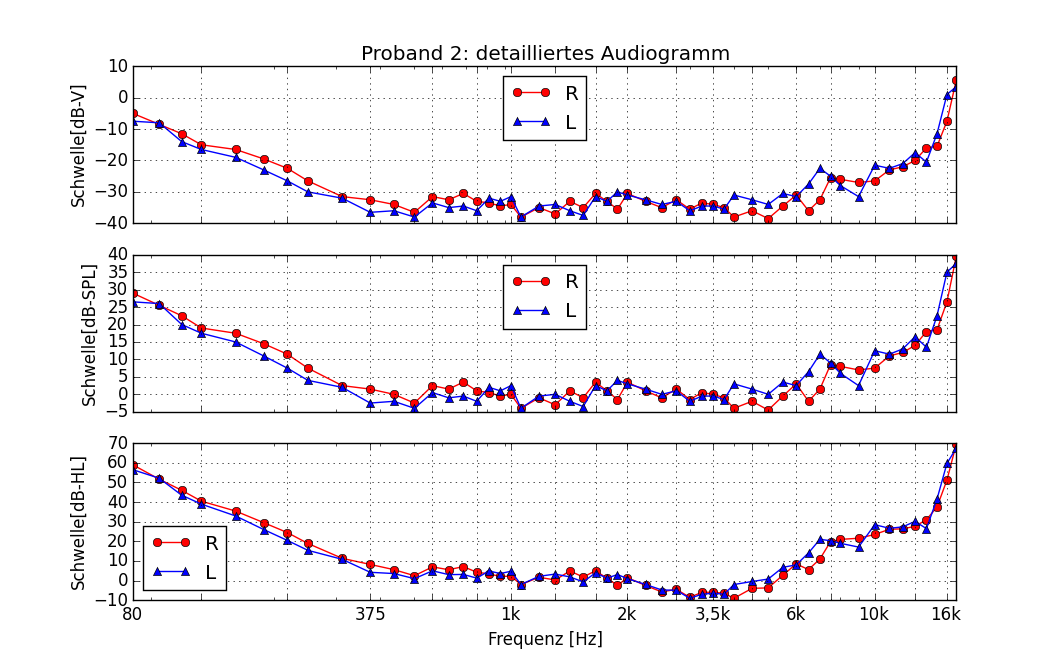
\includegraphics[width=1.\textwidth]{../Bilder/detail_audio.png}
	\caption{Detaillierte Aufl�sung der H�rschwelle von Proband 2 in Abh�ngigkeit der Tonfrequenz in verschiedenen Einheitendarstellungen. Gezeigt sind zun�chst die Signaldaten des Frequenzgenerators (in Einheiten von [dB-V], $\SI{10}{dB-V} \hat{=} \mbox{Signalverdoppelung}$) und darunter die Signaldaten umgewandelt in [dB-SPL] und [dB-HL] (nach Eq. \ref{eq:umrechnung_V-HL}) }
	\label{fig:detail_audio}
\end{figure}


Das Ergebnis dieser Umwandlung ist in Abb. \ref{fig:detail_audio} zu sehen. Man kann erkennen, dass �ber einen breiten Frequenzbereich zwischen ca. $\SI{400}{Hz} < f < \SI{6}{kHz}$, die H�rschwelle nahezu konstant bei $\SI{0}{dB-HL}$ liegt. Zwischen $\SI{2}{kHz}$ und $\SI{4}{kHz}$ sinkt die H�rschwelle sogar auf $\SI{-10}{dB-HL}$ ab. Dies stimmt f�r das linke Ohr mit den Ergebnissen des Audiogramms aus dem ersten Versuchsteil �berein. Es l�sst sich allerdings keine systematische Abweichung zwischen linkem und rechtem Ohr erkennen, was f�r einen Defekt im rechten Kopfh�rer sprechen w�rde, da in diesem Versuch f�r beide Ohren der linke Kopfh�rer verwendet wurde. 
In den Frequenzbereich $f < \SI{400}{Hz}$ und $f > \SI{6}{kHz}$ ist ein Anstieg der H�rschwelle zu verzeichnen. 

\subsubsection{Einfluss von St�rquelle}

\begin{figure}[htbp]
	\centering
		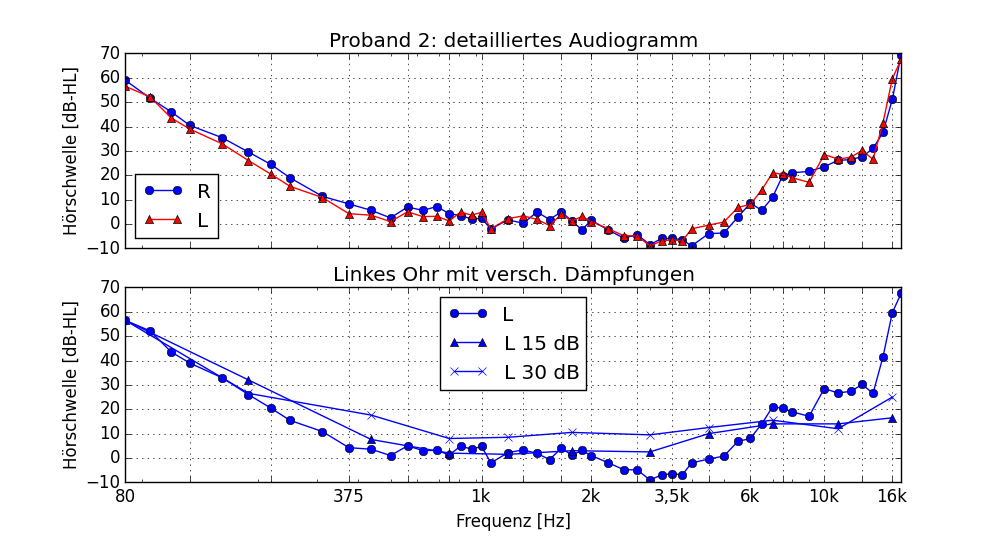
\includegraphics[width=1.00\textwidth]{../Bilder/detail_audio_atten_hl.png}
	\caption{Audiogramm mit St�rgrauschen verschiedener Schallintensit�t. }
	\label{fig:detail_audio_atten_hl}
\end{figure}


Zum Abschluss dieser Versuchsreihe wird der Einfluss einer St�rquelle auf die H�rschwelle des Probanden untersucht. Es wird �ber einen zweiten Funktionsgenerator ein \textit{White-Noise} mit einer Intensit�t von $\SI{15}{dB-SPL}$ (bzw. $\SI{30}{dB-SPL}$) auf das Tonsignal gegeben und erneut ein Audiogramm aufgezeichnet, das ebenfalls nach Eq. \ref{eq:umrechnung_V-HL} umgewandelt wird. Es wurden allerdings weniger Test-Frequenzen als im vorherigen Versuchsteil verwendet und es wurde nur das linke Ohr getestet. Das Ergebnis ist in Abb. \ref{fig:detail_audio_atten_hl} zu sehen. \\
Bei geringem Rauscheinfluss von nur $\SI{15}{dB-SPL}$ ver�ndert sich das Audiogramm von Proband 2 nur minimal, sodass sich die H�rschwelle kaum verndert. F�r das lautere Rauschen von $\SI{30}{dB-SPL}$ ist allerdings zu erkennen, dass eine h�here Signallautst�rke vonn�ten ist, um das eigentliche Signal vom Rauschen zu trennen und den Ton wahr zu nehmen. Die Audiogrammkurve verschiebt sich also nach oben.  

\section{Fazit}

In dieser Versuchsreihe im Rahmen des Praktikums zur Einf�hrung der medizinischen Physik wurden Audiogramme von verschiedenen Probanden mit verschiedenen Messaufbauten aufgenommen und daraufhin erfolgreich miteinander verglichen. Es konnten bekannte Ergebnisse im Rahmen der zur Verf�gung gestellten Aufbauten rekonstruiert werden und der Einfluss von Rauschen auf die H�rwahrnehmung untersucht werden. 

\end{document}
